%--------------------
% Packages
% -------------------
\documentclass[11pt,a4paper]{article}
\usepackage[utf8x]{inputenc}
\usepackage[T1]{fontenc}
%\usepackage{gentium}
\usepackage{mathptmx} % Use Times Font

\usepackage[pdftex]{graphicx} % Required for including pictures
\usepackage[english]{babel} % Swedish translations
\usepackage[pdftex,linkcolor=blue,pdfborder={0 0 0}]{hyperref} % Format links for pdf
\usepackage{calc} % To reset the counter in the document after title page
\usepackage{enumitem} % Includes lists
\usepackage{fancyhdr}
\pagestyle{fancy}

\frenchspacing % No double spacing between sentences
\linespread{1.2} % Set linespace
\usepackage[a4paper, lmargin=0.1666\paperwidth, rmargin=0.1666\paperwidth, tmargin=0.1111\paperheight, bmargin=0.1111\paperheight]{geometry} %margins
%\usepackage{parskip}

\usepackage[all]{nowidow} % Tries to remove widows
\usepackage[protrusion=true,expansion=true]{microtype} % Improves typography, load after fontpackage is selected

\usepackage{lipsum} % Used for inserting dummy 'Lorem ipsum' text into the template

\usepackage{tikz}
\usetikzlibrary{automata,positioning}
\usetikzlibrary{shapes.misc}
\usetikzlibrary{arrows, chains,fit, decorations.text}

\usepackage{algorithm2e}
\RestyleAlgo{ruled}
%% This declares a command \Comment
%% The argument will be surrounded by /* ... */
\SetKwComment{Comment}{/* }{ */}

%-----------------------
% Personal Variables to fill to complete the header
%-----------------------
\newcommand{\HWnum}{T\;} 
\newcommand{\Probnum}{T\;} 
\newcommand{\name}{John Doe\;} 
\newcommand{\netid}{jdoe2\;} 

\fancyhead{}
\fancyhead[L]{\name}
\fancyhead[C]{Homework \HWnum - Problem \Probnum}
\fancyhead[R]{\netid}

\hypersetup{
	colorlinks
}
%-----------------------
% Begin document
%-----------------------
\begin{document} %All text i dokumentet hamnar mellan dessa taggar, allt ovanför är formatering av dokumentet
	
	Some useful links for writing in LaTeX: 
	\begin{itemize}
		\item \url{https://ecealgo.com/resources/Useful-Links.html}
		\item \url{https://ecealgo.com/resources/TikzDocumentation.html}
	\end{itemize}

	You should include citations in footers \footnote{\url{https://tex.stackexchange.com/questions/336704/referring-to-title-of-document-in-hypersetup}}. 
	
	\section{Part A}
	\lipsum[3]
	Here is an example of an Algorithm (Alg \ref{alg:two} taken from Overleaf documentation. \footnote{\url{https://www.overleaf.com/learn/latex/Algorithms}}): 
	
	\begin{algorithm}
		\caption{An algorithm with caption.}\label{alg:two}
		\KwData{$n \geq 0$}
		\KwResult{$y = x^n$}
		$y \gets 1$\;
		$X \gets x$\;
		$N \gets n$\;
		\While{$N \neq 0$}{
			\eIf{$N$ is even}{
				$X \gets X \times X$\;
				$N \gets \frac{N}{2}$ \Comment*[r]{This is a comment}
			}{\If{$N$ is odd}{
					$y \gets y \times X$\;
					$N \gets N - 1$\;
				}
			}
		}
	\end{algorithm}	
	
	\section{Part B}
	Let's also include a TikZ example picture (Figure \ref{fig:tikz}). 
	
	\begin{figure}
		\centering
		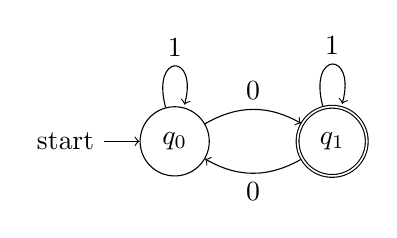
\begin{tikzpicture}
			[->, align=center,node distance=2cm and 4cm] 
			\node[state, initial] (q1) {$q_0$};
			\node[state, accepting, right of=q1] (q2) {$q_1$};
			\draw 
			(q1) edge[loop above] node{1} (q1)
			(q1) edge[bend left, above] node{0} (q2)
			(q2) edge[loop above] node{1} (q2)
			(q2) edge[bend left, below] node{0} (q1);
		\end{tikzpicture}
		\caption{Sample TikZ picture from Lecture 3.}
		\label{fig:tikz}
	\end{figure}
	
	
	\lipsum[5]
	
	
\end{document}
